%@def.tex
\documentclass[a4paper,12pt,oneside]{article}
\usepackage[warn]{mathtext}
\usepackage[T2A]{fontenc}
\usepackage[utf8]{inputenc}
\usepackage[english, russian]{babel}
\usepackage{indentfirst}
\usepackage{amsmath, amsfonts, amssymb}
\usepackage{geometry}
\usepackage{hyperref}
\geometry{top=2cm}
\geometry{left=3cm}
\geometry{right=2cm}
\geometry{bottom=2cm}
\usepackage{graphicx}
\usepackage{epstopdf}
\usepackage{tikz}
\usetikzlibrary{arrows}
\usetikzlibrary{calc}

\renewcommand{\vec}{\overline}
\renewcommand{\phi}{\varphi}

\newenvironment{mintemize}%
{
    \vspace{-0.5em}
    \begin{itemize}
        \setlength\itemsep{-0.2em}
}
{
    \end{itemize}
    \vspace{-0.5em}
}

\graphicspath{{pics/}}


\begin{document}

\begin{cslide}
    \includegraphics[width=3cm]{mai.eps}

    \large\textbf{ Разработка алгоритмов управления
    массивом беспилотных летательных аппаратов
    с целью построения информационного поля
    участка местности}

    \vfill

    \begin{flushright}
    \small Выполнил студент гр. 07-608 Бутко О.А.

    \small Руководитель Жидков В.Н.
    \end{flushright}

    \vfill

    \small Москва, 2015
\end{cslide}

\begin{tslide}{Что такое массив БПЛА}

    Массив БПЛА -- группа однотипны, сверхлёгких, дешёвых БПЛА,
    значительно превышающая по количеству классические группы

    Юнит -- элемент массива БПЛА

    Количество юнитов в системе может исчисляться тысячами
\end{tslide}

\begin{tslide}{Для чего нужен МБПЛА}
\begin{itemize}
    \item построение трёхмерной динамической \newline
        карты неизвестной местности
    \item исследование и построение карты помещений
    \item непрерывный трекинг подвижных объектов
    \item патруль территории
    \item построение дополненной реальности \newline ("взор сквозь стены")
\end{itemize}
\end{tslide}

\begin{tslide}{Для чего нужен МБПЛА}

    \includegraphics[width=\linewidth]{s50s_map2.png}

\end{tslide}

\begin{tslide}{Реализация МБПЛА}
\begin{itemize}
\item Построение информационного поля участка местности
\item Поддержка актуальности, полноты и достоверности информационного поля
\item Обеспечение высокоскоростного канала радиосвязи
\end{itemize}
\end{tslide}

\begin{tslide}{Аспекты реализации}
\begin{itemize}
\item Разделение данных
\item Разделение вычислений
\item Локальная система позиционирования
\item Построение маршрута обхода местности
\item Задача позиционирования в пределах видимости
\item Взаимосвязь и иерархия элементов МБПЛА
\end{itemize}
\end{tslide}

\begin{tslide}{В работе рассматривается}

\begin{itemize}
\item Формализация карты местности
\item Модель юнита, его оснащение и принцип перемещения
\item Алгоритм обхода выпуклых препядствий
\item Алгоритм построения карты местности
    с вариациями
\item Реализация ПМО и проведение экспериментов
\end{itemize}

\end{tslide}

\begin{tslide}{Модель карты местности}

    \includegraphics[width=\linewidth]{map.png}

\end{tslide}

\begin{tslide}{Модель карты местности}

    Предполагается что участок местности ограничен по ширине,
    глубине и высоте.
    Он разбивается на прямоугольные сектора, каждый из которых хранит
    информацию об единице объёма:

    \begin{mintemize}
    \item сколько раз был исследован сектор
    \item когда было произведенно последнее исследование
    \item результат исследования (занят ли сектор)
    \end{mintemize}

    Реализация карты представляет собой 1-мерный массив,
    к которому можно обратиться с помощью трёх индексов-координат.
    Так же для карты имеется матрица трансформации координат
    из локальных (индексов) в глобальные (метры).

\end{tslide}

\begin{tslide}{Модель единицы массива}
    
    \begin{itemize}
    \item За основу была взята концепция БПЛА с вертикальным взлётом
    \item У каждого юнита на борту имеется датчик измеряющий "карту глубин"
        с определённой разрешающей способностью
    \item Каждый юнит знает о положении остальных юнитов системы
    \end{itemize}

    Дифференциальное уравнение движения:
    $$
    \left\{
        \begin{array}{l l}
        \dot{\vec{p}}  & = \vec V \\
        \dot{\vec{V}}  & = \vec a + \vec g
        \end{array}
    \right.
    $$

\end{tslide}
\begin{tslide}{Модель единицы массива}
    
    В список действующих на юнит сил входят:
    \begin{itemize}
    \item Сила сопротивления воздуха
        $$\vec X_0 = C_{x0}\frac{-\vec V \rho |V|}{2} S$$
    \item Коррекция по ближайшим опасным точкам
    \item Управляющее воздействие
    \end{itemize}

    Если сумма сил превышает порог в горизонтальной проекции
    нормируются компоненты $x$ и $y$ совместно, отдельно проверяется
    значение по компоненте $z$.

\end{tslide}

\begin{tslide}{Заполнение карты}

    \begin{itemize}
        \item 1. получаем карту глубин
        \item 2. с помощью обратной матрицы перспективной трансформации
            переводим каждую точку на карте глубин в точку в пространстве
        \item 3. для каждой точки строим отрезок из камеры в эту точку
    \end{itemize}
\end{tslide}
\begin{tslide}{Заполнение карты}
    \begin{itemize}
        \item 4. проходим по отрезку с небольшим шагом
            \begin{itemize}
            \item на каждом шаге приводим точку к системе координат карты
            \item если сектор не исследован помечаем сектор карты как пустой
            \end{itemize}
        \item 5. проверям длину отрезка
            \begin{itemize}
            \item если близко к предельному для сенсора значению по дальности
                то помечаем сектор на конце отрезка как пустой
            \item иначе помечаем сектор как заполненный
            \end{itemize}
    \end{itemize}

\end{tslide}

\begin{tslide}{Коррекция по ближайшим опасным точкам}

    \tikzstyle{every picture}+=[
        axis/.style={black},
        vector/.style={->,line width=1mm,black},
        help/.style={gray,thin,dashed},
        rot/.style={tdplot_rotated_coords}
    ]

    \def\dot{circle[radius=0.5mm]}
    \def\P{1.9}
    \def\Pm{1.6}
    \def\Pmm{0.5}
    \def\Vrot{20}
    \def\fnlen{5}
    \def\ftlen{2}
    \def\dst{8}

    \begin{center}
    \tdplotsetmaincoords{0}{0}
    \begin{tikzpicture}[scale=1.6,tdplot_main_coords]
        \tdplotsetrotatedcoords{85}{60}{-50}
        \fill[rot,red] (\dst,  0,  0) \dot;
        \fill[rot,red] (\dst, .5,  0) \dot;
        \fill[rot,red] (\dst,-.5,  0) \dot;
        \fill[rot,red] (\dst, .5, .5) \dot;
        \fill[rot,red] (\dst,-.5, .5) \dot;
        \fill[rot,red] (\dst,  0, .5) \dot;
        \fill[rot,red] (\dst,  0,-.5) \dot;
        \fill[rot,red] (\dst, .5,-.5) \dot;
        \fill[rot,red] (\dst,-.5,-.5) \dot;

        \fill[rot,black] (0,0,0) \dot node[below] {$O$};

        \draw[rot,vector] (0,0,0) -- (\dst,0,0);
        \node[rot,above] at (6,0,0) {$\vec D$};
        \draw[rot,vector] (0,0,0) -- (1,0,0);
        \node[rot,below] at (1,0,0) {$\vec e_D$};

        \draw[rot,vector] (0,0,0) -- (\Vrot:5) node[above] {$\vec V$};
        \draw[rot,vector] (0,0,0) -- (\Vrot:1) node[above] {$\vec e_V$};
        \draw[rot,vector,help] (0,0,0) -- (0,0,3);
        \node[rot,left] at (0,0,3) {$\vec U$};
        \draw[rot,vector,red] (0,0,0) -- (-\fnlen,0,0);
        \draw[rot,vector,red] (0,0,0) -- (-1,0,0);
        \node[rot,below left] at (-\fnlen,0,0) {$\vec f_N$};
        \node[rot,below] at (-1,0,0) {$\vec N$};
        \draw[rot,vector,green] (0,0,0) -- (0,\ftlen,0);
        \draw[rot,vector,green] (0,0,0) -- (0,1,0);
        \node[rot,above left] at (0,\ftlen,0) {$\vec f_T$};
        \node[rot,above] at (0,1,0) {$\vec T$};
        \draw[rot,vector,blue] (0,0,0) -- (-\fnlen,\ftlen,0);
        \node[rot,above left] at (-\fnlen,\ftlen,0) {$\vec f_{\text{к}}$};

        \draw[rot,help] (0,\ftlen,0) -- ++(-\fnlen,0,0) -- ++(0,-\ftlen,0);

        \draw[rot,help] (0,0,\P) -- ++(0:\P) -- ++(0,0,-\P);
        \draw[rot,help] (0,0,\P) -- ++(\Vrot:\P) -- ++(0,0,-\P);
        \draw[rot,help] (0,\Pm,0) -- ++(\Pm,0,0) -- ++(0,-\Pm,0);
        \draw[rot,help] (-\Pmm,0,0) -- ++(0,\Pmm,0) -- ++(\Pmm,0,0);
    \end{tikzpicture}
    \end{center}

    К ближайшим опасным точкам относятся заполненные сектора карты и
    юниты системы.

    Направление тангенсальной компоненты определяется по текущей скорости.

\end{tslide}

\begin{tslide}{Управляющее воздействие}

    Управляющее воздействие определяется положением целевой
    точки

    Было выбрано 3 вариации выбора целевых точек:
    \begin{itemize}
        \item Распределение по секторам карты подгрупп юнитов
        \item Поиск ближайших неизведанных регионов
        \item Случайный выбор точки в пределах карты
    \end{itemize}

\end{tslide}

\begin{tslide}{Программно-математическое обеспечение}

    В ПМО можно выделить 3 основные части:
    \begin{itemize}
        \item Базовая -- работа с векторами, матрицами, системы
    взаимодействия классов, управление памятью и тд

        \item Графическая -- оконная система, классовые обёртки
            для работы с \verb|OpenGL|

        \item Симуляция МБПЛА
    \end{itemize}

    Гетерогенные вычисления с использованием \verb|OpenCL| нельзя
    полностью отнести к симуляции МБПЛА, так как они тесно связанны
    с графической частью.

\end{tslide}

\begin{tslide}{Программно-математическое обеспечение}

    \centering
    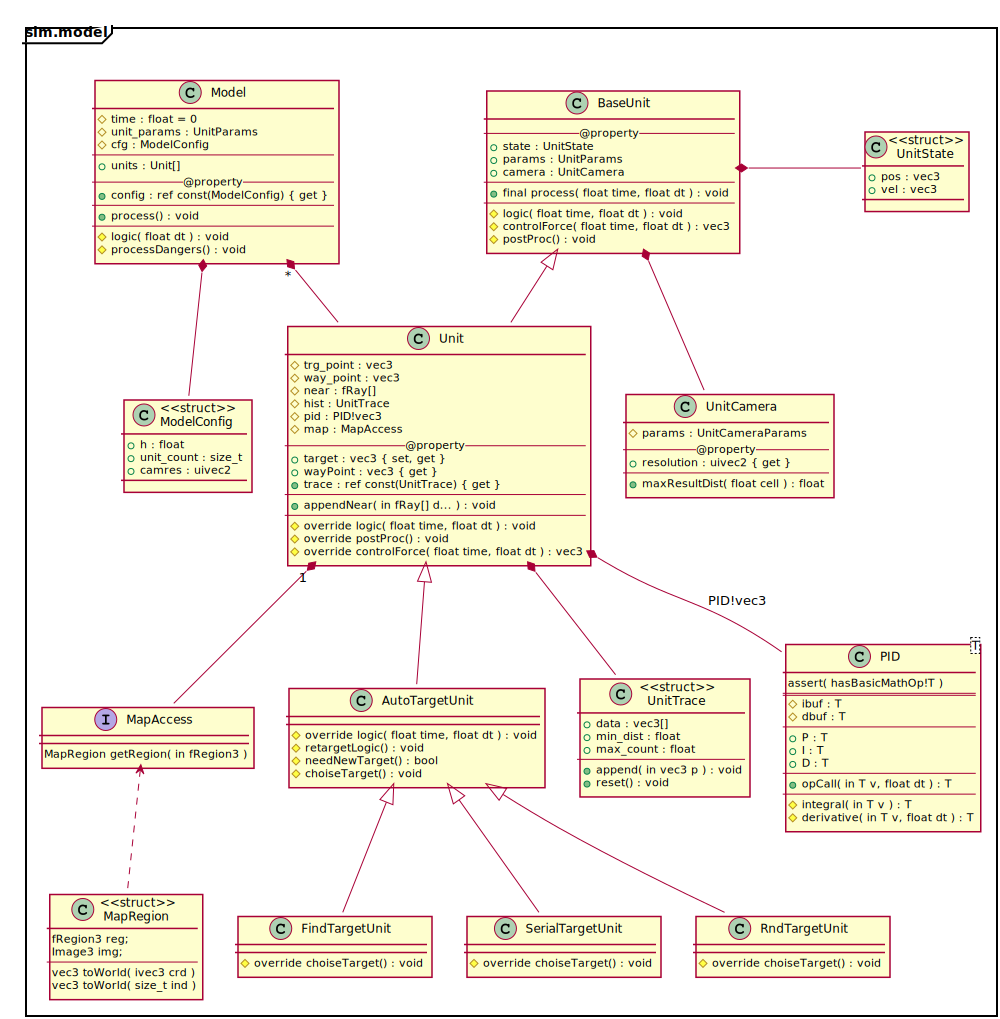
\includegraphics[width=.6\linewidth]{model_uml.eps}

\end{tslide}

\begin{tslide}{Результаты экспериментов}

    \centering
    \includegraphics[width=.9\linewidth]{all_pknown.png}
\end{tslide}

\begin{tslide}{Результаты экспериментов}

    \centering
    \includegraphics[width=.9\linewidth]{all_ts.png}
\end{tslide}

\begin{tslide}{Выводы}

    В процессе выполнения работы были достигнуты поставленные цели:
    \begin{mintemize}
    \item Разработан алгоритм обследования местности
    \item Написано ПМО
    \item Произведены эксперименты
    \item Проанализированы результаты
    \end{mintemize}

\end{tslide}

\begin{cslide}
    \LARGE Спасибо за внимание.
\end{cslide}

\end{document}
